144. \begin{figure}[ht!]
\center{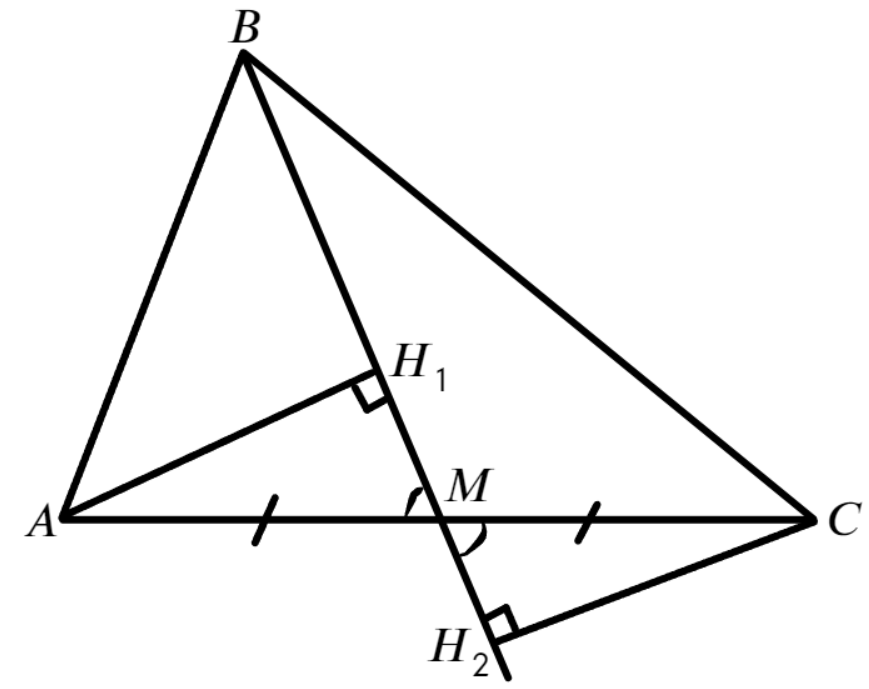
\includegraphics[scale=0.35]{g7-143.png}}
\end{figure}\\
Пусть $BM$ --- медиана, а $AH_1$ и $CH_2$ --- высоты. Углы $AMH_1$ и $CMH_2$ равны как вертикальные, значит прямоугольные треугольники $AMH_1$ и $CMH_2$ равны по гипотенузе и острому углу $(AM=MC),$ значит $AH_1=CH_2,$ ч.т.д.\\
